% !Mode:: "TeX:UTF-8"
\chapter{绪论}
\label{introduction}

\section{课题背景与意义}

2007 年,苹果公司在 Macworld 上展示了第一代 iPhone。
第一台 Android 手机 HTC Dream 也在 2008 年问世。
近几年,智能手机越来越普及,已经进入了寻常百姓的手中,据国际电信联盟统计,截止 2012 年 9 月底,移动互联网用户已经达到 15 亿。
随着设备数量和使用人数的增长,许多互联网上的应用也不断向移动互联网迁移,也有不少在互联晚上难以实现、体现着移动互联网位置相关、实时在线等特征的功能在移动互联网上不断涌现。其中基于地理位置信息的应用不断增多,不论是传统的地图、导航类应用,foursquare、街旁等签到类应用,还是 Yelp、大众点评等本地生活服务类应用,都如雨后春笋般出现。
还有一类应用的数量也在不断上升--交友类应用,得益于移动设备的私密性、易于获取的地理位置信息、随时在线等特性,交友类应用在移动互联网上的活跃程度远高于传统互联网。

本课题是企业课题,是作者在某创业团队实习时的公司项目--“芳邻”,该项目即属于上文提到的交友类应用。

\section{国内外研究现状}

\subsection{手机应用}

手机应用(mobile app)是一种在智能手机、平板电脑和其他移动设备上运行的应用程序。
手机应用一般是通过分发平台来进行安装的,这些分发平台一般由手机操作系统的所有者运行,比如说 Apple App Store、Google Play、Windows Phone Store 和 BlackBerry App World。
其中既有免费应用也有收费应用。
一般来说,手机应用会从商店直接下载到目标设备上,比如 iPhone、黑莓、安卓手机和 Windows Phone,但有时也可以下载到计算机上。
对于收费应用来说,一般会有 20-30\% 的费用会被平台提供商(比如 iTunes)抽走,剩余的部分归 app 的制作者所有。

手机应用原本是为了提高生产力和获取信息而设计的,包括电子邮件、行事历、联系人、股市信息和天气信息等。
然而,大众的需求和必要的开发者工具使得其他类型的应用迅速出现,比如手机游戏,工厂自动化,GPS 和基于地理位置信息的应用,银行,订单管理和购票应用等。
大量多种多样的 app 使得发现优秀的应用成为一种挑战,于是许多评测、推荐、聚合资源,例如博客、杂志和专门的在线应用发现服务。

手机应用正在变得越来越流行。
2012 年 5 月 comScore 的一项研究指出,在上一个季度,手机用户使用移动应用比在他们的设备上浏览网页更多,分别是 51.1\% 和 49.8\%。
研究人员发现手机应用的使用很大程度上被用户所处的环境比如位置和时间所决定。

\subsection{移动互联网}

移动互联网是指通过手持设备,例如智能手机、功能手机或平板电脑,连接到移动网络或其他无线网络上,来访问万维网。

传统上,一般使用大屏幕的手提电脑或桌上电脑通过固定线路来访问互联网。
然而,互联网正在变得越来越易于从手持和无线设备上访问。
一份 2010 年上半年的国际电信联盟的报告指出,移动环境下(通过手提电脑和智能移动设备)的互联网访问的增长率很有可能超过了过去五年中桌上电脑的增长率。
2007 年大屏幕多点触控智能手机、2010 年多点触控平板电脑问世以来,互联网向移动设备迁移的过程大大提速了。
相比上代铲平来说,两个平台都提供了更好的互联网接入、更好的屏幕和手机浏览器或者基于应用程序的互联网体验。网页设计师有时会单独设计移动版页面,或者这些页面会被自动转换来适应移动访问的需要。

移动网页应用和原生应用程序的界限正在变得越来越模糊,现在手机浏览器可以直接访问移动设备的硬件(包括加速度计和 GPS 信息),并且网页应用的速度和能力也得到了提升。
持久化存储和构建复杂用户界面的能力也会使开发平台特定的原生应用的必要性进一步降低。

移动互联网接入现在仍然存在互操作性和可用性的问题。
互操作性问题是由移动设备、操作系统和浏览器的碎片化引起的。
可用性问题主要是源于手机的物理尺寸大小(显示器分辨率和用户输入和操作的先知)。
尽管有这些缺点,许多移动开发者选择在移动互联网上开发应用。
2011 年 6 月的一项针对移动开发的研究发现,移动 web 成为占有率第三的平台,紧随 Android 和 iOS。

在 2013 年 4 月 ACM 通讯的一篇文章中,web 技术专家 Nicholas C. Zakas 指出 2013 年的手机比 1969 年 6 月阿波罗 11 号登月时使用的阿波罗导航计算机计算能力更强。
不过,虽然现在手机的计算能力很强大,2013 年移动设备仍然遭受着和 1996 年相似的 web 性能问题和较慢的连接速度
移动设备有着较慢的下载请求/回应时间,无线数据传输的延迟较大。
“高延迟、较慢的 CPU 和较小的内存”使得开发者不得不重新思考那些为“有线连接、较快的 CPU 和近乎无限内存”的桌面电脑开发的 web 应用程序。

移动互联网增速,是指通过手机、笔记本电脑等设备访问互联网的增速。根据 Tomi Ahonen 的说法,手机接入的增速比其他任何消费品的增速都快。
自这篇文章发布之后,不少文章宣称世界上半数人口已经拥有了手机。
2007\~2008 年间的这些文章有略微的误导性,因为实际情况是在线的手机数量达到了世界人口的一半。
例如,在香港、意大利和乌克兰,手机的占有率已经超过了 140\%(来源:无线智能 2009)。
到 2009 年,手机唯一用户数量也达到了地球人口的一半,ITU 报告手机在网用户已经达到 46 亿,38 亿台手机正在使用,34 亿唯一用户。
移动互联网数据连接跟随手机用户数量一同增长,尽管增速较慢。
2009 年,扬基集团报告说全球手机用户中的 29\% 正在使用浏览器访问互联网。
2010 年,BBC 报道说手机用户数量已经超过 50 亿。

\begin{figure}[h!]
    \centering
    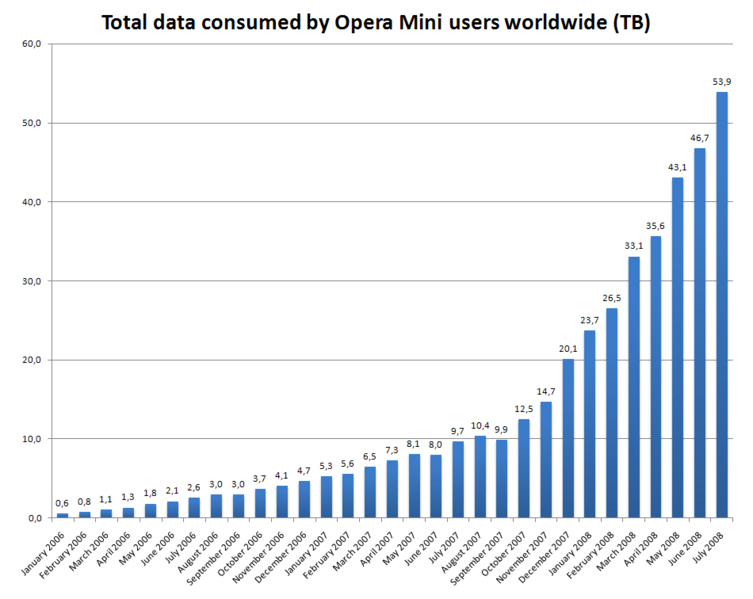
\includegraphics[width=400pt]{figure/Total_data_consumed_by_Opera_Mini_users_worldwide_(TB).png}
    \caption{Opera Mini 全部用户的数据消耗统计}
    \label{opera-mini-total-data}
\end{figure}

\subsection{原生应用与 HTML5}

HTML5 应用在移动领域的魅力不言而喻:
它基于 Web、在移动浏览器内运行,不受移动平台及设备的限制,也不需要开发者针对每个移动操作系统分别开发,“一次写成,到处运行”是它引以为豪的承诺。
没错,HTML5 在很多时候表现得与原生手段并无二致,但是也有几点原因让它往往无法成为众望所归的“完美方案”:
首先,HTML5 本身面临“碎片化”问题,不同移动浏览器对HTML5应用功能的支持存在差异性。
再者,虽然 HTML5 及其相关 Web 语言—— JavaScript 和 CSS 知名度极高,但是 HTML5 移动应用的开发成本往往并不低,也不能单纯地照搬桌面 Web 应用——它们需要优秀的专业人才,也需要巨大的精力投入。

\begin{itemize}
\item 在用户体验及性能方面,原生应用要超过HTML5应用,理由是HTML5依然不能很好地通过所有移动浏览器访问设备原生功能,在打造图形丰富的用户界面和呈现数据方面也存在局限性。

\item 在跨平台部署成本方面,HTML5要占优势,因为HTML5是Web领域的通用语言,不受设备或操作系统限制。
W3C正在接洽汽车、出版和电视行业的公司以推广Web。

\item 在快速更新和发行控制方面,HTML5胜过原生应用。
HTML5的一大优势是开放性——它基于Web,所以没有任何一家公司(如谷歌、苹果、亚马逊或三星)可以充当“掌门人”、放缓更新或者瓜分应用收入。
不过,HTML5在支持设备厂商推出的创新手机功能时有点慢。

\item 在盈利方面,原生应用更胜一筹。
苹果App Store和谷歌Google Play等原生应用商店优势明显。
而HTML5除了软件开发商各自在线销售应用之外,还没有出现令人信服的盈利模式。

\item 在编程人才数量方面,HTML5占优势。HTML5、Javascript和CSS都是Web领域的通用语言,而相比之下,iOS工程师比较短缺而且开价昂贵。
\end{itemize}

移动云计算公司 Appcelerator 认为原生应用的优势用一个词概括就是:性能。

HTML5 适合那些互动性不太强的应用,例如那些单纯提供网络内容或界面非常简单的应用。
然而,如果沿着互动性斜坡上行,那些互动更多的应用就需要原生手段了。

但是,有些设备功能是 HTML5 做不到的,这往往是因为用户的移动浏览器或浏览器版本不支持HTML5实现那些功能。

这在一定程度上是浏览器“碎片化”的结果——一方面,浏览器市场本身就呈现出“群雄割据”之势;
另一方面,很多智能手机用户(尤其是Android用户)不会及时更新软件。

即便是最新的浏览器,对 HTML5 的支持也并不完善——例如我们在近期的一份分析报告中发现,Android 上的最新版 Chrome 浏览器在虽然支持 98 项 HTML5 功能,但是也不支持 28 项功能。

这种不均衡会影响HTML5的跨平台吸引力,而事实上,大量HTML5开发工作依然是致力于桌面环境的。

Appcelerator 认为 HTML5 总会落后五六年,因为它瞄准的“靶子”是移动的——设备厂商和平台运营商总会推出新的硬件、平台和功能,它们很快就能融入原生应用的开发环境,而 HTML5 不得不跟在后面苦苦追赶。

移动后端服务商 StackMobze 则认为 HTML5 已经开始缩小性能上的差距。然而,HTML5 为何在企业内部应用当中比在面向消费者的应用当中更受欢迎?

一大原因,是企业应用和消费应用对用户体验的不同要求——对于消费应用,iOS 已经树立了“黄金标准”而 Android 也随后效仿:丰富多彩的界面和图形、快捷的捏放操作、流畅的滚动、无缝访问照片库和通讯录等设备功能……

这些都是 HTML5 尚未达到的,不是因为 HTML5 无法实现同样的性能,而是因为“HTML5 的用户界面和用户体验没有真正的标准可言”,因此让很多开发者感到很茫然。
一些开发者试图在HTML5环境下模仿iOS式的用户体验,但并不成功。

在当前的移动终端设备硬件配置和操作系统优化水平的前提下,大部分基于 HTML5 开发的 Web 页面会出现延时加载展示的现象,也就是俗称的卡、慢。
特别是在不同的视图界面切换之间,这种卡和不流畅的现象会尤为严重。
而原生应用不会出现这种情况。
究其根源,在于浏览器解析的运作机制和原生的界面展示机制差异上。如图 \ref{html5-native-comparison} 所示:

\begin{figure}[h!]
    \centering
    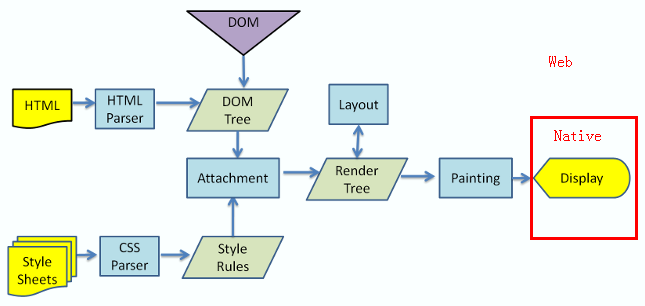
\includegraphics[width=400pt]{figure/html5_native_comparison.png}
    \caption{HTML5 与原生界面展示机制的差异}
    \label{html5-native-comparison}
\end{figure}

红色框起来的部分是原生应用的界面展示机制,简单的看起来就是 1 个步骤——展示,因为所有的绘图和渲染工作都由系统直接完成。
而红框以外的部分包括红框内的部分是 webkit 核心的浏览器解析页面的流程。
相比原生应用的 1 个步骤,webkit 的解析过程可谓漫长而艰辛。
历经解析、建立 DOM 树、获取对应资源、布局、建立渲染树、绘图到展示。
所以不管移动终端设备硬件如何发展,这个差异是始终存在的,最多只是随着硬件的提升和软件的优化将这个差异收缩到最小甚至忽略。

\section{课题研究内容}

本课题的研究内容是设计并实现一款基于地理位置的图片交友应用。
我们遵循开发 iOS 应用的标准流程,并且使用新生的第三方库 -- ReactiveCocoa。
ReactiveCocoa 是由 GitHub 开发的,一个在 Cocoa 框架下的函数式反应型编程(FRP)实现。

\section{论文组织结构}

第 \ref{introduction} 章绪论中,对本文阐述的课题进行说明,主要包括课题的背景、国内玩研究现状、课题研究内容等。

第 \ref{demand} 章需求分析中,详细描述了系统的功能性需求和非功能性需求。

第 \ref{related-technologies} 章相关原理与技术中,对本文所用到的相关技术,如 iOS,ReactiveCocoa,FRP 等进行了详细的阐述。

第 \ref{system-design} 章系统总体设计中,对系统的架构设计进行了介绍,并对其中比较重要的模块进行了详细的描述,例如摇一摇、附近卡片、排行榜、私信等模块。

第 \ref{detail-design-implent} 章系统详细设计与实现中,对一些典型模块的详细设计和实现作了阐述,还附带了具体实现代码,这些模块包括照片的详细信息、排行榜等。

第 \ref{test} 章系统测试评估中,对应用进行了系统的测试,并附上测试用例,测试结果基本符合原本的设计需求。

最后对全文进行了总结。

\chapter{需求分析}
\label{demand}

本课题是一个企业课题,这个课题产生的背景是交友类应用在中国的不断发展。
陌陌等陌生人交友应用的活跃使得我们认识到交友是一个巨大的需求。
目前中国的城市化进程越开越快,人口流动越来越频繁,城市中熟悉的人越来越少,陌生人比例越来越高。
越来越多人的感情和生理需求得不到满足,陌生人之间的交友越来越成为一种必要。

但陌陌等应用虽然提供了陌生人之间相互认识、相互交流的渠道。
但是由于用户没有一个向附近的非特定的陌生人展示自己的方法,使得陌生人之间的交流缺乏话题。
我们的想法是给用户一个向附近非特定的陌生人展示自己的方式,考虑过文字、图片和声音这三种在移动平台上比较容易实现的方式之后,我们选择了图片的方式。
主要原因是图片的生成和浏览都比较简单,在移动设备上,摄像头是标准配置,而网络带宽的增长和 3G、Wi-Fi 连接的普及使得浏览图片相比以前方便便宜了很多。
相比之下,在移动设备上输入文字一直是一个比较耗时的操作,也比较容易出现错误,使得用户趋向于输入较短的文字,或者不输入文字。
声音虽然易于生成,但是声音信息的读取却比其他类型的信息更耗时,声音信息的读取一般来说要与声称耗费同样的时间。
所以我们最终选择了使用图片作为载体,具体分析需求如下。

\section{功能性需求}

本文所述的手机应用,主要包括了照片的拍摄和浏览,对照片的赞和评论,照片信息的用户登录和信息编辑等功能。

系统用例图如图 \ref{use-case-diagram} 所示。

\begin{figure}[h!]
    \centering
    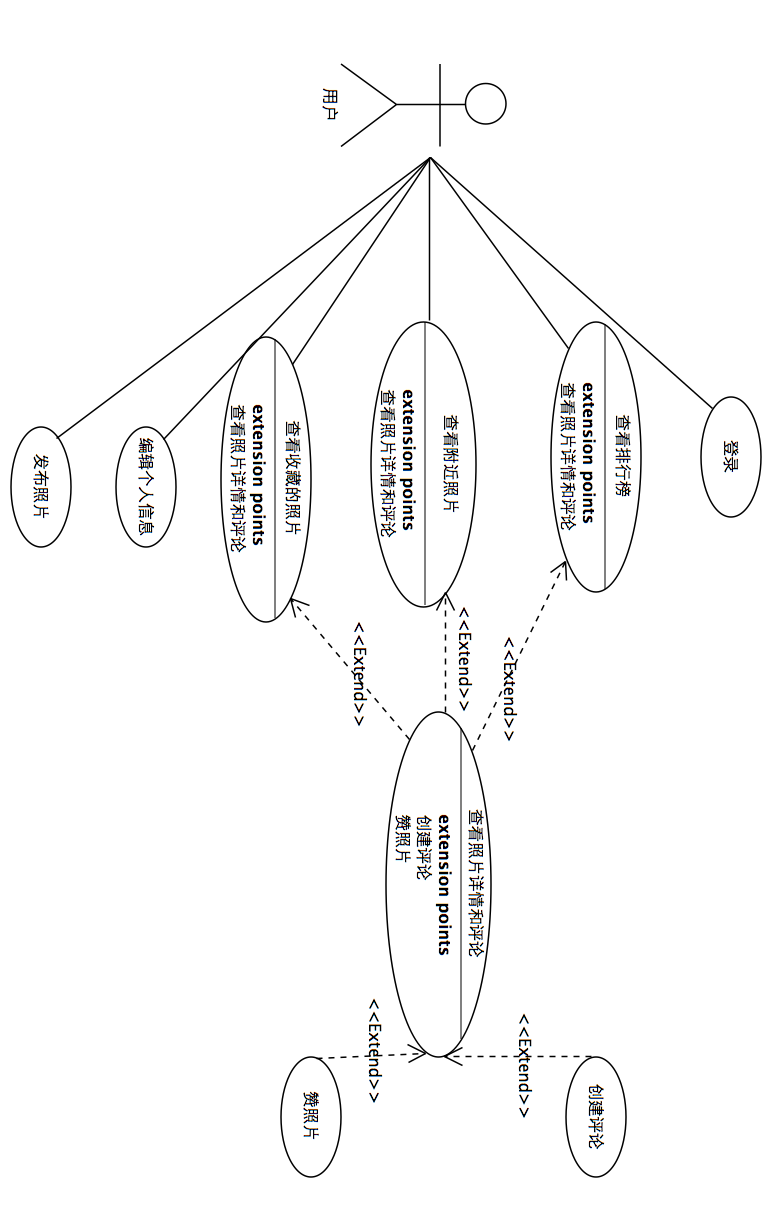
\includegraphics[width=400pt]{figure/use_case_diagram.png}
    \caption{系统用例图}
    \label{use-case-diagram}
\end{figure}

\subsection{登录}

登录是本系统的一个重要需求,所有对系统内的数据进行修改的操作都需要在登录后进行。
例如发布新的照片,对现有照片进行评论等操作均需要在登录后进行。
传统的账号系统的登录方式是采用邮箱、密码的组合进行的,这种方式需要用户在使用之前进行注册,输入邮箱和密码等。
之后再进行登录,再次输入邮箱和密码。
考虑到本系统主要在手机上进行操作,而在手机上输入邮箱和密码是比较麻烦的操作,可能会使比较多的用户放弃注册。
所以我们决定采用第三方登录的方式,在考察了我们的目标用户分布之后,我们选择了新浪微博和 QQ 作为第三方登录方式。

新浪微博的 iOS SDK 提供了与 Facebook 相似的登录方式,通过跳转到微博应用进行登录。
通过这种方式,用户可以不输入任何用户名密码即可完成登录,只需点击允许授权的按钮即可。
这样可以使得用户登录的成本变得比较低,减少因为需要注册、登录而流失的用户数量。

\subsection{查看附近照片}

查看附近照片是系统内获取内容的主要方式。

用户通过这种方式能比较轻易地获取周围其他人的最新动态,也能够跟其他人进行互动,对方便地了解附近其他人的动态有非常重要的意义。
该部分的照片的排序应当综合考虑发布时间距当前时间的时间流逝、照片的热度如评论数量、赞的数量等,对照片进行一个综合排序,该排序应当在服务器端完成。
这是因为,只有服务器端才拥有整个系统内的所有数据,能够对数据进行综合的考虑,对数据进行排序等操作。

服务器的排序过程不需要十分精准,但应当使得客户端得到的数据基本做到不重不漏,在翻页的过程中应当尽量少的出现漏掉照片的情况。
对于在翻页时重复出现的照片,用户不希望看到重复的内容,客户端应当进行过滤,对第二次出现的照片进行合并或删除。
服务端应当提供能够唯一识别某张照片的方式,例如提供唯一 ID 等方式。
客户端应当根据服务器提供的唯一 ID 对照片进行唯一化处理,对重复的照片进行移除等操作,以保证用户看到的照片不会出现重复的情况。

对于服务器的排序算法,应当根据运营中的实际情况进行灵活改变,但是应当遵循一些基本的原则,例如活跃程度更高的照片出现在更前面,发布时间更新的出现在更前面等等。
对于系统运行的初期,可以将活跃程度占的权重适当增大,这样才能在比较稀疏的照片流中突出活跃程度较高的那些。
也可以将排序算法设计成自适应的,从而减少人工调整的必要性。
通过这种方式,可以使得用户查看到用户比较想要看到的结果,该算法还应当通过运营中分析用户的使用习惯进行改进。

\subsection{查看排行榜}

查看排行榜是获取系统内最近的优质内容的一种方式。

本应用中的照片的排行榜是对最近比较大范围内的最近一段时间的优质内容的展示,排行榜中更重视对活跃度较高的照片的展示。
排行榜的存在很重要的一个意义是使得用户对系统内的内容有信息,在系统运行初期,应用内的内容较少,用户遇到高质量内容的机会也就更少。
在这种情况下,通过一定的技术手段使得高质量内容能够有更大可能性得到展示是很重要的。
在系统运行初期,我们选择了比较小的范围进行实验,所以在系统运行过程初期,我们在排行榜中并不限制地域,只是在时间上进行一定的限制。
这样可以避免一些活跃度过高的照片长时间占用排行榜的宝贵空间。

通过这种方式,用户可以更快地获取到系统内的优质内容,对提高用户的粘性,避免用户对系统内的内容产生失望的情绪,避免用户流失应当有着比较好的效果。

\subsection{修改个人资料}

本系统中需要一些个人资料来进行用户相关信息的展示。
这就需要允许用户进行修改等操作。

这些个人资料,对于用户展示自己,吸引其他人的注意有比较重要的意义。
这些信息主要包括用户的昵称,用户的头像和个人介绍等。

为了避免用户信息不全对用户造成的困扰,也为了不占用用户太多的时间对自己的个人信息进行填充,我们要求能够充分利用第三方登录带来的用户信息。
通过新浪微博和 QQ 提供的一些信息来在我们的系统中的用户资料等信息。

除了提供从第三方导入用户资料的功能外,系统还应提供用户手动修改资料的功能,提供修改用户昵称、头像和用户描述信息的功能。
用户昵称为较短的文本,用户描述信息是相对较长的文本,对于它们应当针对它们的特性提供不同的编辑方式。
对于头像只需要一个相对简单的拍照和从已有照片选择的功能,这部分并不需要像创建照片时一样比较复杂的照片编辑等功能,只需要实现比较基本的功能就可以了。

\subsection{查看已收藏的照片}

查看已收藏的照片是指,用户可以对某张照片进行收藏操作,收藏的结果可以在一个专门的页面中进行浏览和编辑等操作。

这些被收藏的照片是用户按照自己的喜好进行选择的,这些照片对于特定用户来说相对比较重要。
所以提供给每个用户查看他们收藏过的照片的方式,通过这样的方式可以使用户持续关注想要关注的照片,对用户粘性有比较大的重要性。

\section{非功能性需求}

\subsection{性能需求}

要求应用程序在 iPhone 4 上不出现明显的卡顿,包括滑动包含大量图片的列表时。

这是因为 iPhone 4 的硬件相对老旧,而在市场上还有一定占有率,我们在选择支持平台的时候选择了支持 iPhone 4 以上硬件。
iPhone 4 的内存比较小,在一些比较耗费内存的操作,比如说展示大量照片、对视频流进行实时处理时会比较吃力,甚至出现崩溃或者被操作系统杀掉等现象。
我们的应用中应当尽量避免这种现象的产生,对不必要的资源尽早进行释放,对视频流进行降低分辨率等处理,使得它们消耗比较少的系统资源。

\subsection{可靠性需求}

要求应用程序尽可能少地崩溃,包括由于占用内存过多而被 iOS 杀掉。

应当通过一定的工具来追踪生产环境中用户的崩溃情况,包括必要的技术信息,用以调试以提高可靠性。
这些信息包括但不限于用户使用的机器类型、用户使用的操作系统版本、用户崩溃时的程序调用栈等,这些信息应该能能够提供一种比较方便的查看方式和调试方式。
特别的,程序的调用栈应当能够提供与源码相关的调试信息,比如源码中的行号,源代码的版本等信息。

\subsection{网络需求}

要求应用程序考虑网络带宽消耗,使用包括缩略图在内的方法来减少带宽消耗。

\section{小结}

本章给出了本文所述系统的需求,包括功能性需求和非功能性需求,功能性需求给出了系统用例图。

\chapter{相关原理与技术}
\label{related-technologies}

\section{iOS}

iOS (之前称作 iPhone OS)是由苹果公司开发和使用的手机操作系统。
原始版本是 2007 年随 iPhone 发行,现在已经扩展到其他苹果设备,例如 iPod Touch、iPad 和 Apple TV(第二代)。
与微软的 Windows Phone 和 Google 的 Android 系统不同的是,苹果并没有把 iOS 授权给非苹果设备使用。
截止 2013 年,苹果的 App Store 中已经有超过 775,000 款 iOS 应用,其中的 300,000 为 iPad 专门优化过。
所有这些应用总共被下载了超过 500 亿次。
2012 年第四季度,iOS 在手机操作系统中占有 21\% 的份额,仅次于 Android。
2012 年 6 月,iOS 设备在全部手机上网流量中占 65\%。
截止 2012 年上半年,共有 4.1 亿设备被激活。
在 2012 年 9 月 12 日苹果召开的特别媒体活动中,苹果公司披露说截止 2012 年 6 月,iOS 设备共卖出 4 亿台。

iOS 使用一种基于直接操作、使用多点触控手势的用户界面。
界面空间元素包括滑块、开关和按钮。
用户与 iOS 的交互手势包括滑动、点击、缩放,这些手势在 iOS 操作系统和多点触控界面中有特定的定义。
一些应用使用内置的加速度计来响应用户摇晃手机(通常会撤销操作)和旋转手机(通常会在竖屏和横屏之间进行切换)。

iOS 来源于 OS X,他们共享同一个 Darwin 内核。
iOS 是苹果电脑上使用的 OS X 的移动版本。

在 iOS 中存在四层抽象:核心操作系统层,核心服务层,媒体层和 Cocoa Touch 层。

\begin{figure}[h!]
    \centering
    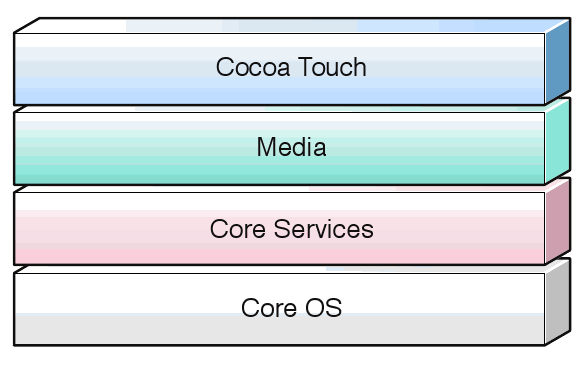
\includegraphics[width=400pt]{figure/iOS.png}
    \caption{iOS 操作系统架构}
    \label{ios}
\end{figure}

核心操作系统层是用 FreeBSD 和 Mach 所改写的 Darwin, 是开源、符合 POSIX 标准的一个 Unix 核心。
这一层包含或者说是提供了整个 iPhone OS 的一些基础功能,比如:硬件驱动, 内存管理,程序管理,线程管理(POSIX),文件系统,网络(BSD Socket),以及标准输入输出等等,所有这些功能都会通过 C 语言的 API 来提供。
另外,值得一题的是,这一层最具有 UNIX 色彩,如果你需要把 UNIX 上所开发的程序移植到 iPhone 上,多半都会使用到 Core OS 的 API.

Core Services 在 Core OS 基础上提供了更为丰富的功能, 它包含了 Foundation.framework 和 Core Foundation.framework, 之所以叫 Foundation ,就是因为它提供了一系列处理字串,排列,组合,日历,时间等等的基本功能。
Foundation 是属于 Objective-C 的 API,Core Fundation 是属于 C 的 API。另外 Core servieces 还提供了其他的功能,比如:Security, Core Location, SQLite 和 Address Book。
其中 Security 是用来处理认证,密码管理,按安全性管理的;
Core Location 是用来处理GPS定位的;
SQLite 是轻量级的数据库,而 AddressBook 则用来处理电话薄资料的。

Media 层提供了图片,音乐,影片等多媒体功能。
图像分为 2D 图像和 3D 图像, 前者由 Quartz2D 来支持,后者则是用 OpenGL ES。
与音乐对应的模组是 Core Audio 和 OpenAL,Media Player 实现了影片的播放,而最后还提供了 Core Animation 来对强大动画的支持。

最上面一层是 Cocoa Touch,它是 Objective-C 的 API, 其中最核心的部分是 UIKit.framework,应用程序界面上的各种组件,全是由它来提供呈现的,除此之外它还负责处理屏幕上的多点触摸事件,文字的输出,图片、网页的显示,相机或文件的存取,以及加速感应的部分等。

\section{Objective-C}

Objective-C 是一种通用、高级、面向对象的编程语言。
它扩展了标准的 ANSI C 编程语言,将 Smalltalk 式的消息传递机制加入到 ANSI C 中。
它是苹果的 OS X 和 iOS 操作系统,及其相关 API、Cocoa 和 Cocoa Touch 的主要编程语言。

Objective-C 最初源于 NeXTSTEP 操作系统,之后在 OS X 和 iOS 继承下来。
目前主要支持的编译器有 GCC 和 Clang,其中 Clang 被应用于 Xcode 4.0 中。

Objective-C 是非常“实际”的语言。
它用一个很小的、用C写成的运行库,使得应用程序的大小增加很少,与此相比,大部分OO系统需要极大的运行时虚拟机来执行。
Objective-C 写成的程序通常不会比其源代码和库(通常无需包含在软件发布版本中)大太多,不会像Smalltalk系统,即使只是打开一个窗口也需要大量的容量。
由于 Objective-C 的动态类型特征,Objective-C 不能对方法进行内联(inline)一类的优化,使得 Objective-C 的应用程序一般比类似的 C 或 C++ 程序更小。

Objective-C 可以在现存 C 编译器基础上实现(在 GCC 中,Objective-C 最初作为预处理器引入,后来作为模块存在),而不需要编写一个全新的编译器。
这个特性使得 Objective-C 能利用大量现存的 C 代码、库、工具和编程思想等资源。现存 C 库可以用 Objective-C 包装器来提供一个 Objective-C 使用的 OO 风格界面包装。

以上这些特性极大地降低了进入 Objective-C 的门槛,这是 1980 年代 Smalltalk 在推广中遇到的最大问题。

Objective-C 的最初版本并不支持垃圾回收。
在当时这是争论的焦点之一,很多人考虑到 Smalltalk 回收时有漫长的“死亡时间”,令整个系统失去功用,Objective-C 为避免此问题才不拥有这个功能。
某些第三方版本加入了这个功能(尤是 GNUstep),苹果公司也在其 Mac OS X 10.5 中提供了实现。

另一个广受批评的问题是 Objective-C 不包括命名空间机制。
取而代之的是程序员必须在其类型名称加上前缀,由于前缀往往较短(相比命名空间),这时常引致冲突。
在 2007 年,在 Cocoa 编程环境中,所有 Mac OS X 类型和函数均有“NS”作为前缀,例如 NSObject 或 NSButton 来清楚分辨它们属于 Mac OS X 核心;使用“NS”是由于这些类型的名称在 NeXTSTEP 开发时定下。

虽然 Objective-C 是 C 的严格超集,但它也不视 C 的基本类型为第一级的对象。

和 C++ 不同,Objective-C 不支持运算符重载(它不支持 ad-hoc 多态)。亦与 C++ 不同,但和 Java 相同,Objective-C 只容许对象继承一个类型(不设多重继承)。
Categories 和 protocols 不但可以提供很多多重继承的好处,而且没有很多缺点,例如额外运行时间过重和二进制不兼容。

由于 Objective-C 使用动态运行时类型,而且所有的方法都是函数调用(有时甚至连系统调用也如此),很多常见的编译时性能优化方法都不能应用于 Objective-C(例如:内联函数、常数传播、交互式优化、纯量取代与聚集等)。
这使得 Objective-C 性能劣于类似的对象抽象语言(如 C++)。不过 Objective-C 拥护者认为 Objective-C 本就不应应用于 C++ 或 ava 常见的底层抽象,Objective-C 的应用方向是对性能要求不大的应用。

\section{Cocoa Touch}

Cocoa Touch 层包含创建 iOS 应用程序所需的关键框架。上至实现应用程序可视界面,下至与高级系统服务交互,都需要该层技术提供底层基础。
如果应用程序构建于 iPhone SDK 4.0 及其后续版本(且运行于 iOS 4.0 及后续版本操作系统),则点击 Home 键的时候,应用程序不会结束,而是切换到后台。对于大多数应用程序来说,进入后台,它们就会进入挂起状态。让应用程序驻留在后台可以避免以后的重新启动过程,应用程序可以直接将自己激活,这在很大程度上改善了整体用户体验。另外,将应用程序挂起也可以改善系统性能,因为挂起应用程序可以最小化电能使用,并可让前台应用程序获得更多的执行时间。
iOS 3.0 及后续版本的系统中,不管应用程序是否运行,苹果推送通知服务可用于通知用户某个应用程序具有新信息。利用这项服务,您可以向系统推送文本通知,可以触发声音提醒或者在应用程序图标上添加一个数字化标记。这样用户就知道他们应该打开应用程序接收相关信息。
iOS 3.2 引入了手势识别器。手势识别器是一个绑定到视图的对象,用于检测常见的手势类型。将手势识别器绑定到视图后,您可以告诉它某个手势发生的时候执行何种动作。之后,手势识别器就可以对原始事件进行跟踪,根据系统定义的试探方式识别手势。在引入手势识别器前,如果要识别一个手势,您需要跟踪视图的原始触摸事件流,然后再使用复杂的试探方法来判断这些事件是否表示某种手势。

下面部分描述 Cocoa Touch 层包含的框架以及这些框架提供的服务。

\begin{itemize}
    \item Address Book UI 框架(AddressBookUI.framework)是一套Objective-C的编程接口,可以显示创建或者编辑联系人的标准系统界面。该框架简化了应用程序显示联系人信息所需的工作,另外它也可以确保应用程序使用的界面和其他应用程序相同,进而保证跨平台一致性。
    \item iOS 4.0引入了Event Kit UI框架(EventKitUI.framework),它提供一个视图控制键可以展现查看并编辑事件的标准系统界面。Event Kit框架(查看“Event Kit框架”可获得该框架的进一步信息)的事件数据是该框架的构建基础。
    \item iOS 3.0引入了Game Kit框架(GameKit.framework)。该框架支持点对点连接及游戏内语音功能,您可以通过该框架为应用程序增加点对点网络功能。点对点连接以及游戏内语音功能在多玩家的游戏中非常普遍,不过您也可以考虑将其加入到非游戏应用程序。此框架通过一组建构于Bonjour之上的简单而强大的类提供网络功能,这些类将许多网络细节抽象出来,从而让没有网络编程经验的开发者可以更加容易地将网络功能整合到应用程序。
    \item iOS 4.0引入了iAd框架 (iAd.framework)。您可以通过该框架在应用程序中发布横幅广告。广告会被放入到标准视图,您可以将这些视图加入到用户界面,并在合适的时机向用户展现。这些视图和苹果的公告服务相互协作,自动处理广告内容的加载和展现,同时也可以响应用户对广告的点击。
    \item iOS 3.0引入了Message UI框架 (MessageUI.framework)。您可以利用该框架撰写电子邮件,并将其放入到用户的发件箱排队等候发送。该框架提供一个视图控制器界面,您可以在应用程序中展现该界面,让用户通过该界面撰写邮件。界面的字段可以根据待发送信息的内容生成。例如您可以设置接收人、主题、邮件内容并可以在邮件中包含附件。这个界面允许用户先对邮件进行编辑,然后再选择接受。在用户接受邮件内容后,相应的邮件就会放入用户的发件箱排队等候发送。

从iOS5开始,Apple就逐渐致力于标准控件的可自定义化,基本包括颜色,图片等的替换。对于标准控件的行为,Apple一向控制的还是比较严格的。而开发者在做app时,最好还是遵守Apple的人机交互手册来确定控件的功能,否则可能遇到意想不到的麻烦…
iOS6中Apple继续扩展了一些控件的可定义性。对于不是特别追求UI的开发团队或者实力有限的个人开发者来说这会是一个不错的消息,使用现有的资源和新加的API,可以快速开发出界面还不错的应用。

\end{itemize}

\subsection{Core Animation}

Core Animation 可以翻译为核心动画,它为图形渲染和动画提供了基础。
使用核心动画,你只需要设置一些参数比如起点和终点,剩下的帧核心动画为你自动完成。
核心动画使用硬件加速,不用消耗 CPU 资源。其实平时咱们开发的 iOS 应用都在有意无意的使用了核心动画。
动画不会替代 view,而是和 view 一起提供更好的性能。
Core Animation 通过缓存 view 上的内容到 bitmap,这样 bitmap 就可以直接在图形硬件上操作。从而提高了性能。

核心动画的动画类使用基本的动画和关键帧动画把图层的内容和选取的属性动画的显示出来。所有核心动画的动画类都是从 CAAnimation 类继承而来。
CAAnimation 实现了 CAMediaTiming 协议,提供了动画的持续时间,速度,和重复计数。 CAAnimation 也实现了 CAAction 协议。该协议为图层触发一个动画动作提供了提供标准化响应。动画类同时定义了一个使用贝塞尔曲线来描述动画改变的时间函数。例如,一个 匀速时间函数(linear timing function)在动画的整个生命周期里面一直保持速度不变, 而渐缓时间函数(ease-out timing function)则在动画接近其生命周期的时候减慢速度。核心动画额外提供了一系列抽象的和细化的动画类,比如:CATransition 提供了一个图层变化的过渡效果,它能影响图层的整个内容。 动画进行的时候淡入淡出(fade)、推(push)、显露(reveal)图层的内容。这些过渡效 果可以扩展到你自己定制的 Core Image 滤镜。CAAnimationGroup 允许一系列动画效果组合在一起,并行显示动画。

\subsection{Core Data}

对于处理诸如对象生命周期管理、对象图管理等日常任务,Core Data 框架提供了广泛且自动化的解决方案。
它有以下特性。
我们把这些对象(和它们之间的联系)成为对象图。 对象图可大可小,有繁有简。

有时,你可能想要把这样的对象图转化形式,让它们可以被保存到文件中,以使其他的进程或其他的机器可以再次将保存的内容读出,重购对象。 这样的过程常被成之为“归档”(Archiving)。

有些对象图是不完整的——通常称之为局部对象图(partial object graphs)。
局部对象图包含了“占位符”(Placeholder)对象,所谓”占位符“,就是一些暂时无内容的对象,它们将再后期被具体化。
一个典型的例子就是 nib 文件中包含的 File's Owner 对象。

使用Core Data有很多原因,其中最简单的一条就是:它能让你为Model层写的代码的行数减少为原来的50\%到70\%。 这归功于之前提到的Core Data的特性。
更妙的是,对于上述特性你也既不用去测试,也不用花功夫去优化。
Core Data拥有成熟的代码,这些代码通过单元测试来保证品质。应用Core Data的程序每天被世界上几百万用户使用。通过了几个版本的发布,已经被高度优化。 它能利用Model层的信息和运行时的特性,而不通过程序层的代码实现。 除了提供强大的安全支持和错误处理外,它还提供了最优的内存扩展性,可实现有竞争力的解决方案。不使用Core Data的话,你需要花很长时间来起草自己的方案,解决各种问题,这样做效率不高。

除了 Core Data 本身的优点之外,使用它还有其他的好处: 它很容易和 Mac OS X 系统的工具链集成;利用模型设计工具可以按图形化方式轻松创建数据库的结构;你可以用 Instruments 的相关模板来测试 Core Data 的效率并 debug。 在 Mac OS X的 桌面程序中,Core Data 还和 Interface Builder 集成,按照模型来创建 UI 变的更简单 了。 这些功能能更进一步的帮助你缩短设计、开发、测试程序的周期。

\section{ReactiveCocoa}

ReactiveCocoa(RAC)是一个 Objective-C 的函数式反应型编程(Functional Reactive Programming,FRP)。
它提供了创建和转换数值流的 API。

\subsection{函数式反应型编程}
函数式反应型编程 (FRP) 是一种编写相应变化的软件的编程范型。

FRP 构建于值随时间变化的抽象。
FRP 提供信号来捕捉过去、现在和未来的值,而不是在特定的时间捕捉某个值。
我们可以引用、串联、创建这些信号,并根据俄这些信号做出反应。

通过结合不同的信号,我们可以通过声明式的方法来编写软件,而不需要编写代码不断地观察和更新值。
比如说可以直接设置某个文本域一直显示现在的时间,而不是编写一些额外的代码来检查时间然后每秒钟更新这个文本域。

信号可以表示异步操作,就像 future 和 promise 一样。
这大大地简化了异步代码的编写,包括网络操作代码。

FRP 的一大优势是,它提供了一个统一的方式来处理不同类型的异步行为。

\subsection{ReactiveCocoa 的使用场景}

初看起来,ReactiveCocoa 非常抽象,比较难与理解和应用于具体问题。

这里介绍一些 RAC 适用的场景:

\begin{itemize}

\item 操作异步或事件驱动的数据源。

很多 Cocoa 代码都在关注对用户时间和应用程序状态改变做出反应。
这些处理事件的代码会很快地变得非常杂乱,很可能会出现许多回调和状态变量。

有些看起来不同的模式,比如说 UI 回调,网络回应,和 KVO 通知,实际上有很多相同点。
RACSignal 统一了这些 API 以使得他们能用相同的方式来处理。

\item 串联有依赖的操作。

网络请求中经常存在依赖,前一个请求完成之后后一个请求才能被构建。ReactiveCocoa 使得这种情况变得非常简单。

\item 并行化独立的操作。

在 Cocoa 中使独立操作并行执行不是一件非常简单的事情,而且往往伴随着许多同步代码。ReactiveCocoa 使得这些代码变得非常清楚。

\item 简化集合操作。

FoundationKit 中缺少一些一些高阶函数,例如 map、filter、fold/reduce,使得许多基于循环的代码频频出现。
RACSequence 使得我们可以用一种统一的声明式的方法来操作 Cocoa 集合。

\end{itemize}

代码 \ref{reactivecocoa} 给出一段 ReactiveCocoa 的使用示例。

\begin{minipage}{\textwidth}
\begin{lstlisting}[caption=ReactiveCocoa 示例, label=reactivecocoa]
- (void)viewDidLoad {
    [super viewDidLoad];

    @weakify(self);

    RAC(self.logInButton, enabled) = [RACSignal
        combineLatest:@[
            self.usernameTextField.rac_textSignal,
            self.passwordTextField.rac_textSignal,
            RACAbleWithStart(LoginManager.sharedManager, loggingIn),
            RACAbleWithStart(self.loggedIn)
        ] reduce:^(NSString *username, NSString *password, NSNumber *loggingIn, NSNumber *loggedIn) {
            return @(username.length > 0 && password.length > 0 && !loggingIn.boolValue && !loggedIn.boolValue);
        }];

    [[self.logInButton rac_signalForControlEvents:UIControlEventTouchUpInside] subscribeNext:^(UIButton *sender) {
        @strongify(self);

        RACSignal *loginSignal = [[LoginManager sharedManager]
            logInWithUsername:self.usernameTextField.text
            password:self.passwordTextField.text];

        [loginSignal subscribeError:^(NSError *error) {
            @strongify(self);
            [self presentError:error];
        } completed:^{
            @strongify(self);
            self.loggedIn = YES;
        }];
    }];
}
\end{lstlisting}
\end{minipage}

\chapter{系统总体设计}
\label{system-design}

\section{架构设计}

本系统的架构主要由三个层次构成:界面与业务逻辑、模型层、网络层。如图 \ref{architecture} 所示。

\begin{figure}[h!]
    \centering
    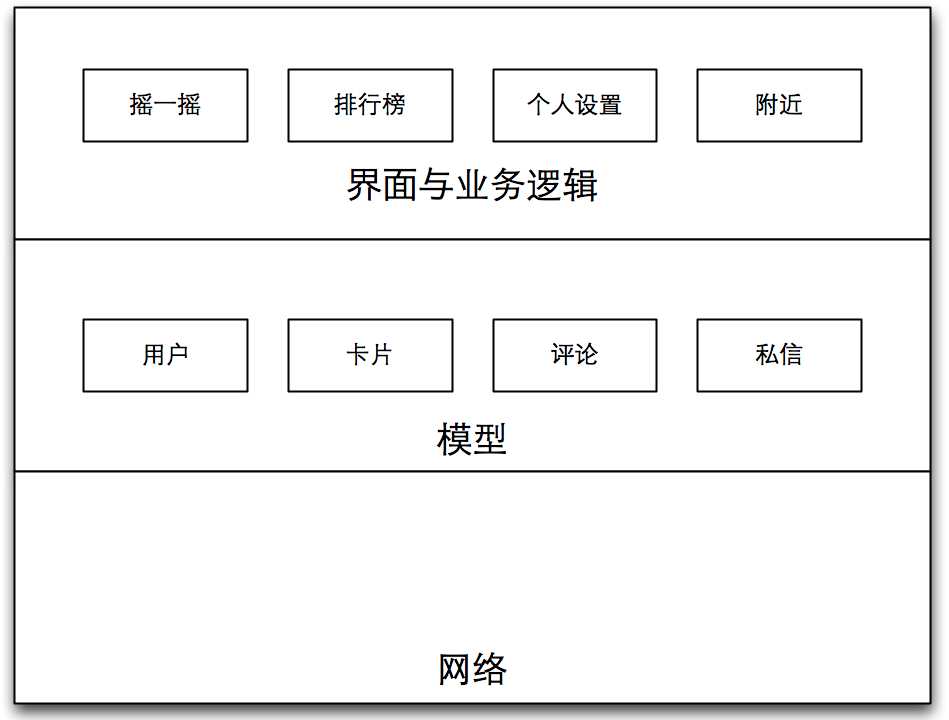
\includegraphics[width=400pt]{figure/architecture.png}
    \caption{系统架构图}
    \label{architecture}
\end{figure}

界面与业务逻辑层主要提供用户可见的用户界面与具体的业务逻辑。
界面主要包括,用户可以看到的视图,包括图片,交互按钮,动画等内容。
业务逻辑主要包括用户做出操作之后的系统应当进行的相应,包括调用下层的模型及网络层,对视图做出相应的修改等。
合并页面(视图)与业务逻辑(控制器)是 Cocoa 开发中的惯例。
这是因为在 iOS 中,视图与控制器的耦合比较深,对于一个 iOS 应用来说,很大一部分是在对视图进行操作。
业务逻辑中经常穿插着对视图的操作,例如显示载入指示,进行实际的载入,隐藏载入指示,刷新视图。
如此紧密的耦合使得区分它们的开销变得很大,会使代码变得非常复杂。

模型层主要由一些模型类构成,他们完成了对系统中的实体的创建、修改、查看、删除等操作,并且会调用网络层对服务器上的相关资源进行调用。
这部分使用 Core Data 完成,所以这些模型类都是 NSManagedObject 的子类,他们通过 Core Data 进行持久化,后端使用 SQLite 进行存储。实体关系图如图 \ref{entity-relationship-diagram} 所示。

\begin{figure}[h!]
    \centering
    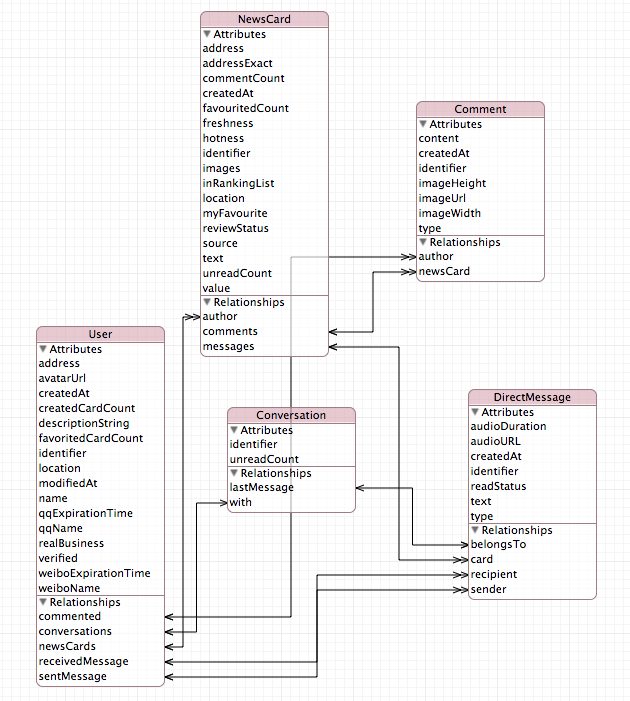
\includegraphics[width=400pt]{figure/entity_relationship_diagram.png}
    \caption{实体关系图}
    \label{entity-relationship-diagram}
\end{figure}

网络层主要由一个网络服务类构成,它将服务器的 API 包装成 Objective-C 接口。
网络层基于 AFNetworking 进行构建,主要内容是一个 AFHTTPClient 的子类,他完成了对服务器提供的 HTTP 接口的封装。
客户端与服务器通过基于 HTTP 和 JSON 的 API 进行沟通。

\section{摇一摇模块}

摇一摇模块使得用户可以通过摇晃手机来获得随机的照片,获得的照片由服务器上特定的算法选定。
该模块的顺序图如图 \ref{shake-device-sequence-diagram} 所示。

\begin{figure}[h!]
    \centering
    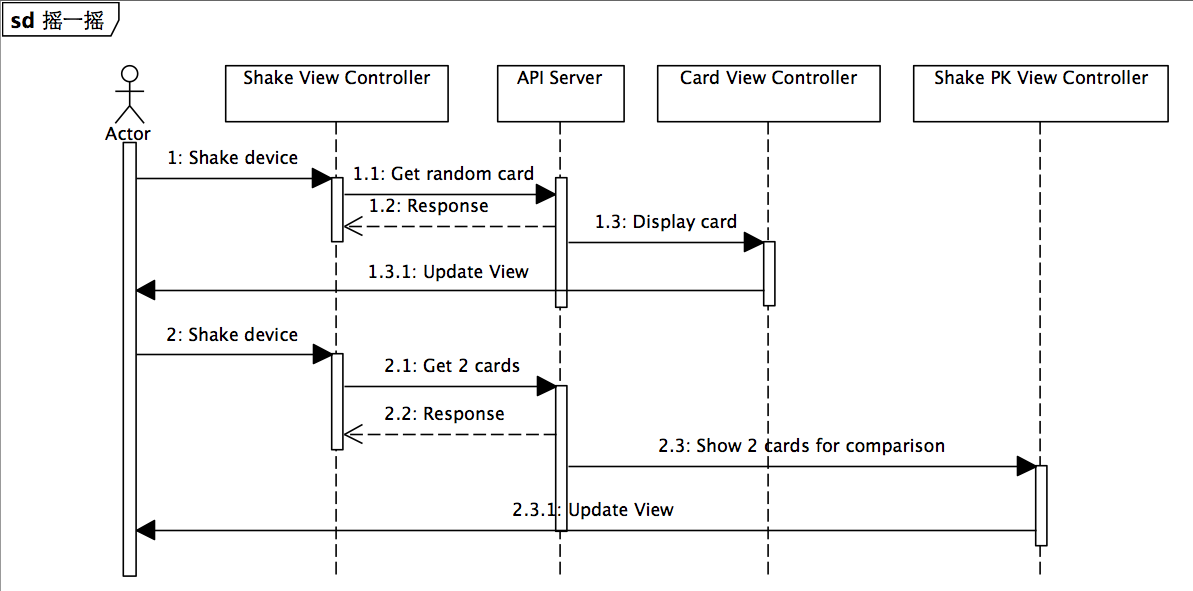
\includegraphics[width=400pt]{figure/shake_device_sequence_diagram.png}
    \caption{摇一摇模块顺序图}
    \label{shake-device-sequence-diagram}
\end{figure}

\section{附近卡片模块}

附近卡片模块实现附近卡片的浏览和评论功能。
该模块的顺序图如图 \ref{nearby-cards-sequence-diagram} 所示。

\begin{figure}[h!]
    \centering
    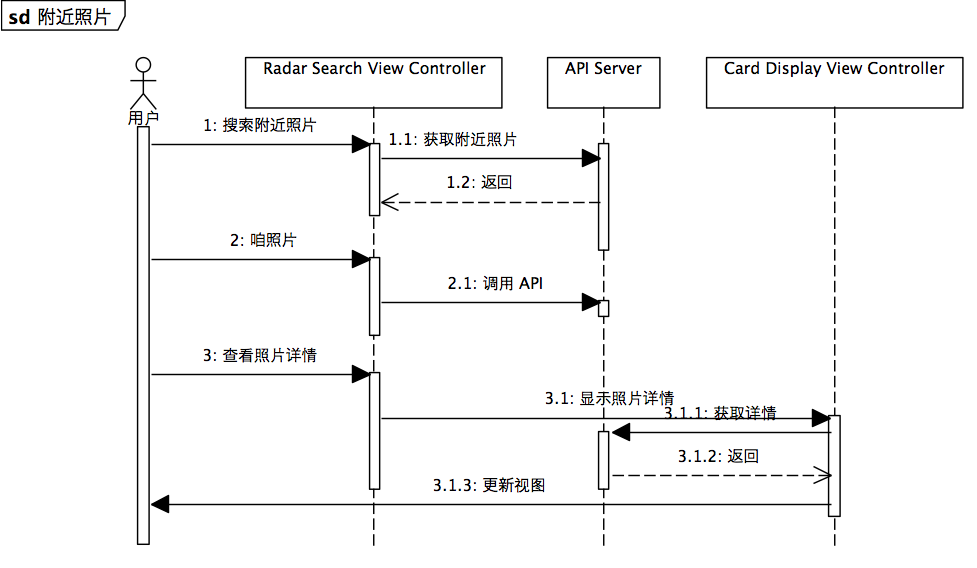
\includegraphics[width=400pt]{figure/nearby_cards_sequence_diagram.png}
    \caption{附近卡片模块顺序图}
    \label{nearby-cards-sequence-diagram}
\end{figure}

\section{排行榜模块}

排行榜模块实现浏览最新的照片排行榜功能。
该模块的顺序图如图 \ref{rank-list-sequence-diagram} 所示。

\begin{figure}[h!]
    \centering
    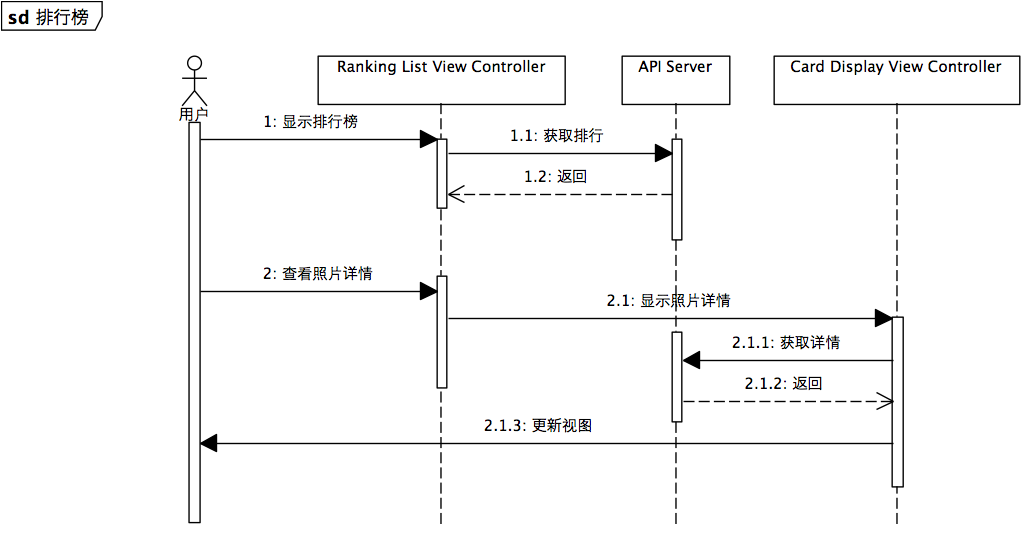
\includegraphics[width=400pt]{figure/rank_list_sequence_diagram.png}
    \caption{排行榜模块顺序图}
    \label{rank-list-sequence-diagram}
\end{figure}

\section{私信模块}

私信模块实现两个用户之间的即时通讯功能,它的功能与其他即时通讯功能相差不多,主要用于两个用户有初步的认识之后进行进一步交流。
该模块的设计与其他带有即时通讯功能的软件相差不多,在此不详细描述。

\chapter{系统详细设计与实现}
\label{detail-design-implent}

本章将详细介绍本系统的设计与实现。
本章将论述本系统中三部分--界面与业务逻辑、模型层和网络层--的一些详细的设计,例如类的关系,采用的技术,使用的设计模式等,以及这样设计的原因。

由于这是一个商业系统,所以其中技术上同质化的部分比较多,对于这些部分,将选取比较典型的几个来进行论述。

\section{照片详细信息的展示和交互}
\label{photo-detail}

这部分是作者在本应用中最早实现的一部分,这部分功能实现了照片本身和相关信息的展示,另外还包括与照片相关的交互。
信息包括照片的发布者的昵称、头像,照片的收藏数字,照片发布位置距当前位置的距离,照片发布位置的 POI 信息,照片相关的评论等信息。

这个视图的展示与逻辑主要是由 FRNewsCardDisplayViewController 这个类实现的。
这个类是 UIViewController 的子类,如同他的名字暗示的那样,它实现了相关的视图和控制器的功能。
它负责将照片和相关内容展示出来,并且负责响应用户的操作。
效果示例如图 \ref{card-detail} 所示。

\begin{figure}[h!]
    \centering
    
\includegraphics[width=320pt]{figure/card_detail.png}
    \caption{照片详细信息示例图}
    \label{card-detail}
\end{figure}

效果图中可以看出,该视图上半部分是关于照片的一些信息,例如照片本身的图片,附属的文字,作者的昵称和头像,创建图片时的位置,与用户当前位置的距离等。
下半部分(图 \ref{card-detail} 中未显示)还有该照片所属的评论信息,包括评论作者的头像、昵称、评论的内容和发表评论的时间,以列表的形式显示。
由于这些需求的存在,FRNewsCardDisplayViewController 在最外层视图中添加一个 UIScrollView 来包含整个内容,包括照片相关信息和评论的列表。
照片相关的信息由类 FRNewsCardViewController 来负责展示和交互,这是因为,照片信息的这种展示形式在整个应用中反复出现,并非只有在本视图中出现。
因此,遵循 DRY(Do not repeat yourself)的原则,考虑到代码复用,而将这个部分独立出来。

但在 view controller 中内嵌 view controller 是一个相对较新的技术,它在 iOS 5 中首次出现,应当格外注意添加的方式,否则可能会出现内嵌的 view controller 不能正确相应一些事件的情况。相关的代码如代码 \ref{nested-view-controller} 所示。

\begin{minipage}{\textwidth}
\begin{lstlisting}[caption=嵌套 view controller, label=nested-view-controller]
[self addChildViewController:_newsCardViewController];
[_contentView addSubview:_newsCardViewController.view];
[_newsCardViewController didMoveToParentViewController:self];
\end{lstlisting}
\end{minipage}

头像的圆形遮罩和阴影的实现也有一定的技巧,为了实现的简单,作者选择不使用 Quartz 2D 遮罩的方式,而是采用一个半径大小的圆角来实现。
代码如 \ref{avatar} 所示。

\begin{minipage}{\textwidth}
\begin{lstlisting}[caption=头像的阴影和遮罩的实现, label=avatar]
_avatarImageView = [[UIImageView alloc] initWithFrame:CGRectMake(12, CGRectGetMaxY(_imageContainer.frame) - 14, 40, 40)];
_avatarImageView.backgroundColor = [UIColor whiteColor];
_avatarImageView.layer.borderWidth = 2;
_avatarImageView.layer.borderColor = [[UIColor whiteColor] CGColor];
_avatarImageView.layer.cornerRadius = 20;
_avatarImageView.layer.masksToBounds = YES;
[self.view addSubview:_avatarImageView];
\end{lstlisting}
\end{minipage}

在照片信息之后,是评论的列表,这是一个 UITableView 的子类,它负责评论内容的显示和更新。
它由若干个 FRNewsCardCommentCell 组成,每个 FRNewsCardCommentCell 用来显示一条评论。
但由于滚动事件由外层的 scroll view 接管,该 table view 并没有接受滚动事件,导致该 table view 不能进行单元格的复用。
这样会导致在评论比较多的时候生成比较多的 FRNewsCardCommentCell,致使内存占用比较多,程序出现卡顿等。
这说明该类还需要进行重构,主要是将最外层的视图替换成一整个 table view,而不是 scroll view。
照片的信息作为 table view 的一个 section 来提供,这样 table view 的 cell 复用功能就能正常运作了。

\section{排行榜的显示和交互}

排行榜是应用中比较晚制作的功能,分析了之前的设计出现的问题,吸取了教训,排行榜的设计和代码都比较成熟。
所以作者用排行榜来描述应用中非常常见的列表的场景。
排行榜的示例图如图 \ref{ranking-list} 所示。

\begin{figure}[h!]
    \centering
    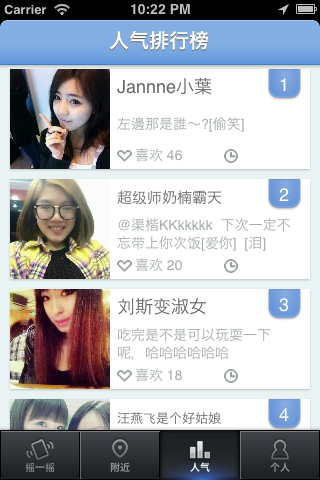
\includegraphics[width=320pt]{figure/ranking_list.png}
    \caption{排行榜示例图}
    \label{ranking-list}
\end{figure}

排行榜的页面使用了 AFHTTPClient 的一个子类来进行网络请求,该类的单例对象在请求回当前排行榜的数据之后,对数据进行解析,生成一系列排行榜相关的对象,放入 Core Data 中。
之后使用 NSFetchedResultsContoller 读取存放在 Core Data 中的信息。

使用 NSFetchedResultsContoller 有不少好处。
首先,它是有苹果提供的,与 Cocoa Touch 框架结合更紧密。
另外他使用 Core Data 中的数据,使用 NSFetchRequest 进行查询。
这样就能利用已经在 Core Data 中的数据和 Core Data 提供的各种功能强大的设施,使得 Core Data 和 table view 很好地结合起来。
例如说 NSFetchRequest 可以指定需要查询的实体种类,通过指定谓词的方式指定查询条件,谓词是由 NSPredicate 表示的,它的形式有点类似 SQL。
NSFetchedResultsContoller 的最大的一个好处就是可以使得视图的展示得到实时的更新而不需要显式的再次查询 Core Data。
也就是说,每次我们获得了新数据,或者删除、修改了老的数据,通过 NSFetchedResultsContoller,能够实时地在视图上反映出来,而不用编写额外的代码。

NSFetchedResultsController 的核心其实是作为一个观察者去监听 NSManagedObjectContext 的通知。当 NSManagedObjectContext 发生改变的时候 NSFetchedResultsController 就知道了变化。
所以,我们初始化 一个NSFetchedResultsController 的时候,也就监听了对应的 NSManagedObjectContext 的通知。
具体的是三个通知:NSManagedObjectContextObjectsDidChangeNotification、NSManagedObjectContextWillSaveNotification 和 NSManagedObjectContextDidSaveNotification。

\begin{itemize}
    \item NSManagedObjectContextObjectsDidChangeNotification
当任何一个对象中的任何属性有改变的时候,会发出此通知。然后 NSFetchedResultsController 会去用设置好的 NSFetchRequest 查处结果进行参数传递。当这些改变发送的时候,我们就只用在 -controller:didChangeObject:atIndexPath:forChangeType:newIndexPath:判断改变类型是 NSFetchedResultsChangeUpdate 或者 NSFetchedResultsChangeMove 就可以做相应的数据到 UI 的变更操作了。
    \item NSManagedObjectContextWillSaveNotification
这个通知是在删除对象的情况下。 这时候可能删除的是 section。用 -controller:\-didChangeSection:\-atIndex:\-forChangeType:。 如果只是一个对象的删除。就用 -controller:\-didChangeObject:\-atIndexPath:\-forChangeType:\-newIndexPath:。
类型都是 NSFetchedResultsChangeDelete.
    \item NSManagedObjectContextDidSaveNotification
这个通知对应的 delegate 方法就是 -controller:\-didChangeSection:\-atIndex:\-forChangeType: 和 -controller:\-didChangeObject:\-atIndexPath:\-forChangeType:\-newIndexPath:。
\end{itemize}

NSFetchedResultsController 的示例可以在附录 \ref{nsfetchedresultscontroller} 找到,该示例是在联系人列表界面中节选的,主要原因是联系人列表界面逻辑比较简单。

在排行榜中比较大量地使用了 ReactiveCocoa,主要用来保证数据的一致性。
从截图中可以看出,排行榜中每个照片都存在喜欢数量、发布时间等信息,这些信息可能随着用户的操作发生改变。
为了保证这些数据在整个应用中的一致性,作者使用了 ReactiveCocoa,如代码 \ref{ranking-rack} 所示。

\begin{minipage}{\textwidth}
\begin{lstlisting}[caption=排行榜中的数据绑定,label=ranking-rack]
@weakify(self);
[RACAbleWithStart(self.imageURL) subscribeNext:^(NSURL *imageURL) {
    @strongify(self);
    [self.photoImageView setImageWithURL:imageURL];
}];
[RACAbleWithStart(self.name) subscribeNext:^(NSString *name) {
    @strongify(self);
    self.nameLabel.text = name;
}];
[RACAbleWithStart(self.content) subscribeNext:^(NSString *contentString) {
    @strongify(self);
    self.contentLabel.text = contentString;
}];
[RACAbleWithStart(self.rank) subscribeNext:^(NSNumber *rank) {
    @strongify(self);
    self.rankingLabel.text = [NSString stringWithFormat:@"%d", [rank integerValue]];
}];
[RACAbleWithStart(self.likeCount) subscribeNext:^(NSNumber *likeCount) {
    @strongify(self);
    self.likeCountLabel.text = [NSString stringWithFormat:@"喜欢 %d", [likeCount integerValue]];
}];
[RACAble(self.date) subscribeNext:^(NSNumber *timeInterval) {
    @strongify(self);
    NSDate *date = [NSDate dateWithTimeIntervalSince1970:[timeInterval integerValue]];
    self.dateLabel.text = [NSDateFormatter relativeTimeStringFromNow:date];
}];
\end{lstlisting}
\end{minipage}

ReactiveCocoa 采用了 FRP 的编程范型。这类似于设计模式中的观察者模式,实现上也基于 Cocoa 中的 KVC(Key-Value Coding) 与 KVO(Key-Value Observing)。在此种模式中,一个目标对象管理所有相依于它的观察者对象,并且在它本身的状态改变时主动发出通知。这通常透过呼叫各观察者所提供的方法来实现。此种模式通常被用来实现事件处理系统。

在观察者模式的实现中,采用了一种叫做 isa swizzling 的技术。
大体上来说,它是将被观察的对象的类型改变,插入一个观察者代理对象,由该代理对象执行观察者模式要求的行为。
这也就是说在实现 KVO 的同时,使用了另一种设计模式,代理模式。

\section{摇一摇}

摇一摇主要实现在检测到用户摇晃设备之后,随机显示一张照片。
显示照片的部分可以使用 \ref{photo-detail} 照片浏览部分的功能,所以该模块的主要难点就是检测设备的摇晃。

设备摇晃可以用 UIResponder 的 -motionBegan:withEvent: 方法进行检测,但要格外注意的是,这个方法的调用是沿着 responder chain 进行传递的。
在iOS系统中,能够响应并处理事件的对象称之为 responder object, UIResponder 是所有 responder 对象的基类,在 UIResponder 类中定义了处理各种事件,包括触摸事件(Touch Event)、运动事件(Motion Event)和远程控制事件(Remote-Control Events)的编程接口。

第一响应者(first responder) 是处于一个应用程序中的响应者对象(通常是一个 UIView 对象),该对象被指定为非触摸事件的第一个接收者。
一个 UIWindow 在消息中给第一响应者发送这些事件,给它处理过程中的第一镜头。
要接收这些消息,响应者对象必须实现 -canBecomeFirstResponder 并返回 YES;它还必须接收一个 becomeFirstResponder 消息(可以自我触发)。

响应链是一个响应者对象的连接序列,事件或动作消息(或菜单编辑消息)依次传递。
它允许响应者对象把事件处理的职责转交给其它更高层的对象。
应用程序通过向上传递一个事件来查找合适的处理对象。
因为点击检测视图也是一个响应者对象,应用程序在处理触摸事件时也可以利用响应链。

iOS 中的响应链如图 \ref{responder-chain} 所示。

\begin{figure}[h!]
    \centering
    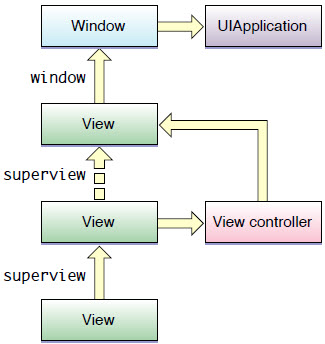
\includegraphics{figure/responder_chain.jpg}
    \caption{响应链}
    \label{responder-chain}
\end{figure}

\begin{enumerate}
    \item 点击检测视图或者第一响应者传递事件或动作消息给它的视图控制器如果它有的话;如果没有一个视图控制器,就传递给它的父视图(superview)。

    \item 如果一个视图或者它的视图控制器不能处理这个事件或动作消息,它将传递给该视图的父视图。

    \item 在这个视图层次中的每个后续的父视图遵循上述的模式,如果它不能处理这个事件或动作消息的话。

    \item 最顶层的视图如果不能处理这个事件或动作消息,就传递给UIWindow对象来处理。

    \item 如果UIWindow 对象不能处理,就传给单件应用程序对象UIApplication。

    \item 如果应用程序对象也不能处理这个事件或动作消息,将抛弃它。
\end{enumerate}

\section{Badge Keeper}

iOS 应用在桌面上的图标可以显示一个红色圆形底白色字的数字指示,叫做 badge number,应用经常使用这个数字来显示未读信息。
应用的其他地方也用到了同样意义的数字,但是这些数字的来源不同,有些是通过苹果的推送服务获得的,有些是从 API server 获取的,并且还有可能根据用户的操作改变。
原始的设计是每个控制器维护自己的数字,但这样不可避免的造成维护的困难和不一致性。
所以后来将这个功能抽取出来作为一个单独的类 -- FRUnreadCountKeeper。
这个类虽然代码很短,但是它的设计比较好,具有正交性、只有单一职责,也考虑了线程安全等问题,所以选择它在本文中进行展示,见代码 \ref{unread-count-keeper}。

\begin{minipage}{\textwidth}
\begin{lstlisting}[caption=FRUnreadCountKeeper 的实现, label=unread-count-keeper]
@implementation FRUnreadCountKeeper

static FRUnreadCountKeeper *_sharedKeeper;

+ (instancetype)sharedKeeper {
    static dispatch_once_t onceToken;
    dispatch_once(&onceToken, ^{
        _sharedKeeper = [[FRUnreadCountKeeper alloc] initPrivate];
    });
    return _sharedKeeper;
}

- (void)setUnreadCount:(NSUInteger)unreadCount {
    _unreadCount = unreadCount;
    dispatch_async(dispatch_get_main_queue(), ^{
        [[UIApplication sharedApplication] setApplicationIconBadgeNumber:_unreadCount];
    });
}

- (void)decreaseUnreadCount:(NSInteger)diff {
    self.unreadCount -= diff;
}

- (instancetype)initPrivate {
    self = [super init];
    if (self) {
        _unreadCount = [[UIApplication sharedApplication] applicationIconBadgeNumber];
    }
    return self;
}

@end
\end{lstlisting}
\end{minipage}

\chapter{系统测试评估}
\label{test}

本章将对本文论述的系统进行测试,包括针对功能性需求和非功能性需求的测试

\section{测试环境}

为保证兼容性,兼容新旧硬件和新旧操作系统版本,本系统必须在几种不同的操作系统和硬件上进行测试,具体见表 \ref{env-spec}。

\begin{table}
    \centering
    \caption{测试环境}
    \label{env-spec}
    \begin{tabular}{c|c}
        \hline
        \multirow{2}{*}{操作系统版本} & iOS 5 \\
                                    & iOS 6 \\ \hline
        \multirow{3}{*}{屏幕分辨率}   & 480x320 \\
                                     & 960x640 \\
                                     & 1136x640 \\ \hline
    \end{tabular}
\end{table}

根据测试要求,我们选取了一些机器进行测试,iPhone 4,iPhone 3GS,iPod Touch 5 等设备进行测试。

\section{系统测试}

在这一部分,将对整个应用进行测试,测试主要由人工的方式来进行。
测试的目的主要是验证应用是否符合了原本的设计需求,是否满足了原本设计的需求。

测试主要用测试用例的方式来描述。

\subsection{摇一摇}

摇一摇显示随机照片是本系统的一个关键功能,它通过随机显示照片的方式发现新的朋友。测试用例见表格 \ref{shake-device}。

\begin{table}
    \centering
    \caption{摇一摇的测试用例}
    \label{shake-device}
    \begin{tabular}{c|l}
        \hline
        用例名称    & 摇一摇       \\ \hline
        \multirow{2}{*}{测试类型}    & 功能测试     \\
                   & 界面测试     \\ \hline
        \multirow{3}{*}{涉及的需求}  & 摇一摇       \\
                                    & 显示随机照片  \\
                   & 显示照片对比界面 \\ \hline
        \multirow{3}{*}{先决条件}    & 用户打开应用    \\
                                    & 用户切换到摇一摇标签页 \\
                                    & 用户摇晃手机    \\ \hline
        输入                          & 用户做出摇晃手机的操作 \\ \hline
        \multirow{2}{*}{期望输出}    & 显示随机照片显示界面     \\
                                 & 显示照片对比界面   \\ \hline
        \multirow{2}{*}{实际输出}    & 显示随机照片显示界面 \\
                                    & 显示照片对比界面   \\ \hline
        \multirow{2}{*}{评价准则}   & 系统会对用户在摇一摇界面摇晃手机进行相应,显示随机照片界面 \\
                                   & 系统不会对用户在其他界面摇晃手机进行相应 \\ \hline
        \multirow{3}{*}{测试步骤}   & 用户打开应用    \\
                                   & 用户切换到摇一摇标签页 \\
                                   & 用户摇晃手机    \\ \hline
        假设和约束  & 用户的手机可以接受摇晃事件 \\ \hline
    \end{tabular}
\end{table}

\subsection{下拉刷新}

下拉刷新是在 iOS 中的一个常见的交互过程,在本系统中也大量使用了下拉刷新这种操作。测试用例见表格见 \ref{pull-to-refresh}。

\begin{table}
    \centering
    \caption{下拉刷新的测试用例}
    \label{pull-to-refresh}
    \begin{tabular}{c|l}
        \hline
        用例名称    & 下拉刷新       \\ \hline
        \multirow{2}{*}{测试类型}    & 功能测试     \\
                                    & 界面测试     \\ \hline
        \multirow{2}{*}{涉及的需求}  & 显示排行榜       \\
                                    & 排行榜的刷新  \\
        \multirow{3}{*}{先决条件}    & 用户打开应用    \\
                                    & 用户切换到排行榜标签页 \\
                                    & 用户向下拉页面    \\
                                    & 拉动一定距离后松开手指 \\ \hline
        \multirow{2}{*}{输入}       & 用户向下拉动页面 \\
                                    & 用户释放手指 \\ \hline
        \multirow{2}{*}{期望输出}    & 显示载入提示动画     \\
                                 & 页面刷新   \\ \hline
        \multirow{2}{*}{实际输出}    & 显示载入提示动画 \\
                                    & 页面刷新   \\ \hline
        \multirow{2}{*}{评价准则}   & 系统会在用户下拉足够距离并释放后刷新页面的数据 \\
                                   & 系统会在用户下拉不足够距离并释放后无响应 \\ \hline
        \multirow{3}{*}{测试步骤}   & 用户打开应用    \\
                                   & 用户切换到排行榜标签页 \\
                                   & 用户向下拉页面    \\
                                   & 拉动一定距离后松开手指 \\ \hline
        假设和约束  & 设备已联网 \\ \hline
    \end{tabular}
\end{table}

\subsection{拍摄照片}

拍摄照片是在系统中产生照片的方式,只有通过这样社区内的照片才能保持一定的新鲜度。测试用例见表格 \ref{new-photo}。

\begin{table}
    \centering
    \caption{拍摄照片的测试用例}
    \label{new-photo}
    \begin{tabular}{c|l}
        \hline
        用例名称    & 下拉刷新       \\ \hline
        \multirow{2}{*}{测试类型}    & 功能测试     \\
                                    & 界面测试     \\ \hline
        \multirow{2}{*}{涉及的需求}  & 拍摄照片       \\
                                    & 创建照片元信息  \\
        \multirow{1}{*}{先决条件}    & 用户打开应用    \\ \hline
        \multirow{2}{*}{输入}       & 用户点击拍照按钮 \\
                                    & 点击快门按钮 \\ \hline
        \multirow{2}{*}{期望输出}    & 产生一张照片     \\
                                    & 显示元信息编辑页面   \\ \hline
        \multirow{2}{*}{实际输出}    & 产生一张照片 \\
                                    & 显示元信息编辑页面   \\ \hline
        \multirow{2}{*}{评价准则}   & 系统能够成功地拍摄一张照片 \\
                                   & 系统能够切换到元信息编辑页面 \\ \hline
        \multirow{3}{*}{测试步骤}   & 用户打开应用    \\
                                   & 用户点击拍照按钮 \\
                                   & 点击快门按钮    \\ \hline
        \multirow{2}{*}{假设和约束}  & 设备已联网 \\
                                    & 设备有摄像头 \\ \hline
    \end{tabular}
\end{table}

\section{本章小结}
本章对应用进行了测试,通过比较全面的测试用例对系统的各方面进行了评测。基本达到了原本的设计要求。

\chapter*{总结}
\addcontentsline{toc}{chapter}{总结}
本系统是作者在某公司实习时的公司项目。
顺应移动互联网发展的趋势,考虑到移动互联网的实时在线、位置相关等特性,为了满足越来越多的城市人口的交友需求,设计并实现了本应用。
应用实现了查看附近的照片、查看照片排行榜、拍摄新的照片、对照片进行评论等功能,基本满足了原本的需求,实现了原本的设计。

作者在开发过程中,也学习到了许多相关的知识。
\begin{itemize}
    \item 比较全面地学习了 Ojective-C。
    学习了其中的许多概念,例如 category、protocol、property 等概念,学习了 ARC、block 等新技术,还研究了运行时编程等底层技术。
    \item 学习了 GitHub 编写的 ReactiveCocoa 库,这是一个 FRP 在 Cocoa 中的实现,同时也了解了 FRP 的相关技术,了解了 Elm、Ex 等相关技术。
    \item 对 Cocoa Touch 有了比较深入的了解。
    对 UIKit 有比较深入的了解,明白了 UIViewController 和 UIView 及其常见子类的行为。
    对 Core Data 有一定了解,了解 NSFetchedResultsController、NSFetchRequest、NSPredicate 等配套设施。
    对 Core Graphics 有一定了解,能够使用 Quartz 2D 绘制简单的图形、阴影等。
    对 Core Animation 有一定了解,能够编写各种动画代码,包括动画组等。
    \item 对设计模式有了更深的认识,包括代理模式、单例模式、工厂模式、观察者模式、责任链模式等。
\end{itemize}
